\documentclass[a4paper,11pt,twoside]{article}
%\documentclass[a4paper,11pt,twoside,se]{article}

\usepackage{UmUStudentReport}
\usepackage{verbatim}   % Multi-line comments using \begin{comment}
\usepackage{courier}    % Nicer fonts are used. (not necessary)
\usepackage{pslatex}    % Also nicer fonts. (not necessary)
\usepackage[pdftex]{graphicx}   % allows including pdf figures
\usepackage{listings}
\usepackage{pgf-umlcd}
%\usepackage{lmodern}   % Optional fonts. (not necessary)
%\usepackage{tabularx}
%\usepackage{microtype} % Provides some typographic improvements over default settings
%\usepackage{placeins}  % For aligning images with \FloatBarrier
%\usepackage{booktabs}  % For nice-looking tables
%\usepackage{titlesec}  % More granular control of sections.

% DOCUMENT INFO
% =============
\department{Department of Computing Science}
\coursename{Application Development in Java 7.5 p}
\coursecode{5DV135}
\title{Unit Test Framework}
\author{Lorenz Gerber ({\tt{dv15lgr@cs.umu.se}} {\tt{lozger03@student.umu.se}})}
\date{2016-11-17}
%\revisiondate{2016-01-18}
\instructor{Johan Eliasson / Jan Erik Moström / Alexander Sutherland / Filip Allberg / Adam Dahlgren Lindström}


% DOCUMENT SETTINGS
% =================
\bibliographystyle{plain}
%\bibliographystyle{ieee}
\pagestyle{fancy}
\raggedbottom
\setcounter{secnumdepth}{2}
\setcounter{tocdepth}{2}
%\graphicspath{{images/}}   %Path for images

\usepackage{float}
\floatstyle{ruled}
\newfloat{listing}{thp}{lop}
\floatname{listing}{Listing}



% DEFINES
% =======
%\newcommand{\mycommand}{<latex code>}

% DOCUMENT
% ========
\begin{document}
\lstset{language=C}
\maketitle
\thispagestyle{empty}
\newpage
\tableofcontents
\thispagestyle{empty}
\newpage

\clearpage
\pagenumbering{arabic}

\section{Introduction}
The aim of this assignment was to learn building a simple GUI application, using the Java Reflection class and formatting the source code according to a given code convention. The implemented application is a so called Unit Tester. It runs unit tests on a given class. The unit tests themselves are also defined in a specific class. A screnshot of the running application can be seen in \textit{figure 1}.  

\begin{figure}[p]
    \centering
    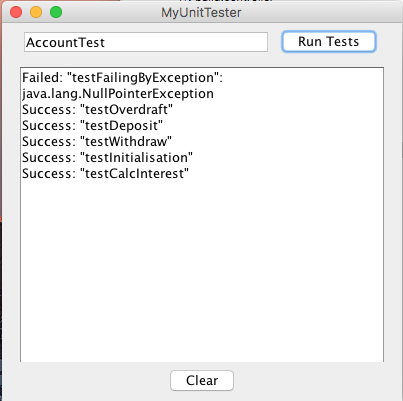
\includegraphics[width=0.8\textwidth]{screenshot.png}
    \caption{This figure shows a typical screendump of the UnitTest applicaiton running on OSX}
    \label{fig:screenshot}
\end{figure}

\section{Usage} 
\subsection{Compiling from Command Line}
The source code for the Java application 'UnitTest' was divided into the packages `model', `view' and `controller'. The class containing the `main' method, the classes to be tested as well as the test classes where contained in the base directory (or default package). The following steps were conducted to build a jar application file:
\begin{verbatim}
mkdir build
javac -d ./build *.java controller/UnitTestController.java ./
    model/*.java view/*.java
cd build
jar cvfe UnitTest.jar UnitTestMain *.class controller/ view/ model/
\end{verbatim} 
Note that the `jar' file is named `UnitTest' while the `main' containing class is named `UnitTestMain'.
The source code is provided in a separate tar.gz file.

\subsection{Program Usage}
The `UnitTest' application is invoked from the command line by \verb+java -jar UnitTest+. Then the application GUI should open with a default test class `Test1' already chosen. To run the unit tests, the user presses the button `Run Tests' upon the output shows up in the main text area. An additional button under the main text area `clear' can be used to empty the main text output area. The application shall be terminated by closing the main application window using the system's window close button.

\section{System Description}
The application was designed according to the Model-View-Controller principle. The following textual description is also represented in an UML model shown in \textit{figure 2}. The model is represented by the UnitTest class. Plugged into a command line only main program, this class provides all functionality needed to do unit testing according to the specifications in the assignment description. Output in this case is obtained through an ArrayList<String> that contains all test messages.
The `view' implementation is the `Swing' based graphical user interface in the class UnitTestGui. Here, it was chosen to keep all interfacing parts to the model such as action listeners outside. Instead, methods that export the interactive elements of the GUI were implemented.
The final part is the UnitTestController class which interconnects model and view. It takes a gui object as argument, which provides the needed access to the GUI elements. The controller class contains all the action listeners and controls the general flow of the program such as verification of the test class and running the actual tests. This is achieved by instantiation of the model from within the controller class.



\begin{figure}[p]
    \centering
    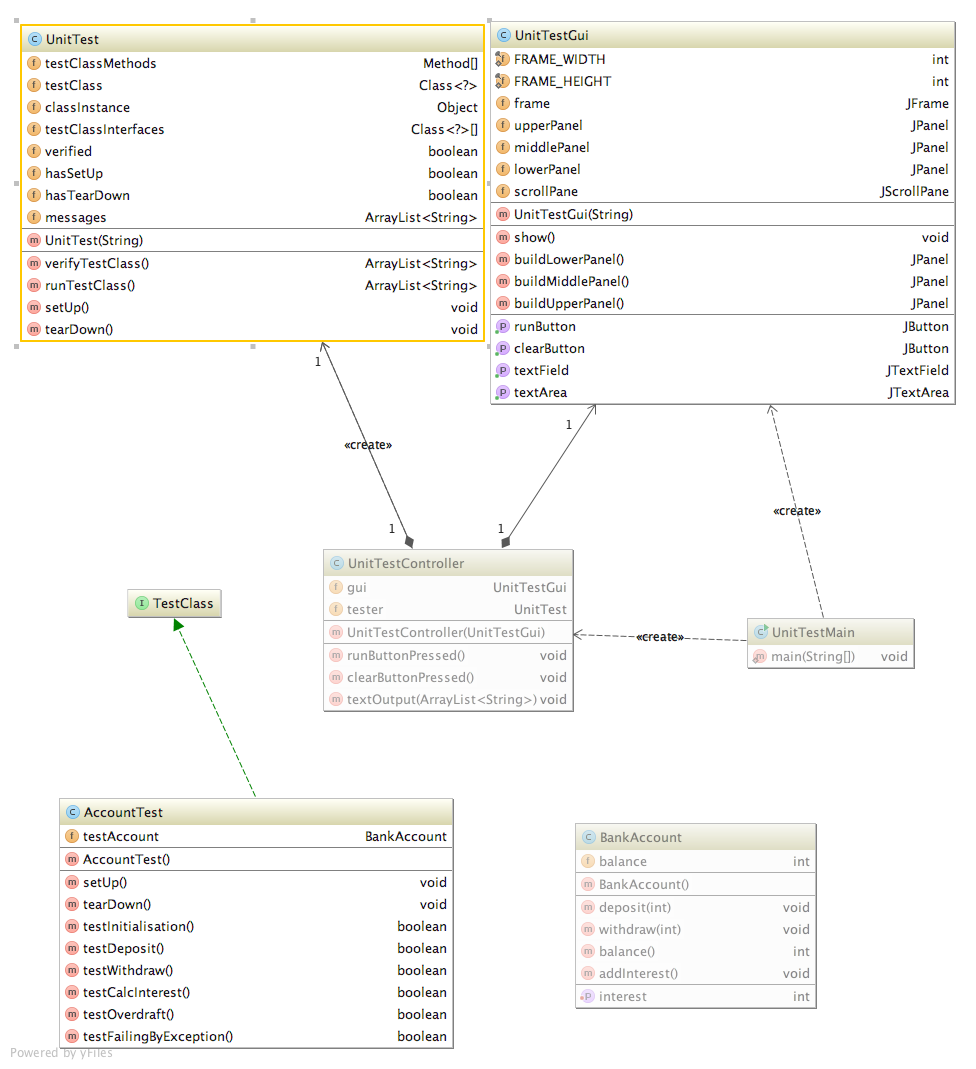
\includegraphics[width=1.2\textwidth]{diagram.png}
    \caption{This figure shows the UML diagram of the UnitTest application.}
    \label{fig:diagram}
\end{figure}


\section{Testing}
A simple class `MyInt' and test class `Test1' was given. One further class with test class had to be implemented additionally. Here 'MyInt' and `Test1' were mostly used to verify the correct functioning of the UnitTest application, while the classes `BankAccout' and `AccountTester' represent more a real world use case. `Test1' contains one case that produces an exception which has to be handled by the UnitTest framework.

Further it was tested whether a wrong test class name would be caught and handled gracefully, i.e. informing the user and going back to base state where the user can enter another test class. This seemed to work, however one special case was then found that could not be handled: If the user enters the correct name of a test class, however with wrong upper/lowercase letters, it is not caught by the usual exception handling. Some search on the web showed that this behaviour could be different between different operating systems based on case sensitivty of the respective file system. I conducted tests on OSX where wrong case, but existing names resulted in uncaught exceptions in the java console. The user interface does not give any clue why nothing happens, however, at least it does not crash and can still be used if a correct test class name is provided. 


\addcontentsline{toc}{section}{\refname}
\bibliography{references}

\end{document}
